% !TEX TS-program = pdflatex
% !TEX encoding = UTF-8 Unicode

% This file is a template using the "beamer" package to create slides for a talk or presentation

\documentclass{beamer}


\mode<presentation>
{
	%%%%%%%%%%%%%%%%%%% use this theme %%%%%%%%%%%%%%%%%%%
  %\usetheme{Warsaw}
  % or ...

  \setbeamercovered{transparent}
  % or whatever (possibly just delete it)
}


\addtobeamertemplate{navigation symbols}{}{%
    \usebeamerfont{footline}%
    \usebeamercolor[fg]{footline}%
    \hspace{1em}%
    \insertframenumber/\inserttotalframenumber
}

\usepackage[english]{babel}
\usepackage{amssymb, amsmath}
% or whatever
\usepackage{graphicx}
\usepackage{subcaption}
\usepackage[utf8]{inputenc}
% or whatever

\usepackage{amsfonts} 
\usepackage{array}

\newenvironment{conditions}
  {\par\vspace{\abovedisplayskip}\noindent\begin{tabular}{>{$}l<{$} @{${}={}$} l}}
  {\end{tabular}\par\vspace{\belowdisplayskip}}
  
\title[Implicit Preferences] % (optional, use only with long paper titles)
{Epidemiological Modelling of Coronavirus Infection in Quarantined Population}

\subtitle
{A Outline of Project for MATH371 Wi2020}

\author[natasha]{Natasha Ting[5mm]{\footnotesize Instructor: Jay Newby}}
%\author[] % (optional, use only with lots of authors)
%{Natasha Ting\inst{} \and %\inst{2}
%}
% - Give the names in the same order as the appear in the paper.
% - Use the \inst{?} command only if the authors have different
%   affiliation.

\institute[University of Alberta] % (optional, but mostly needed)
{
  \inst{}%
  Department of Mathematical and Statistical Sciences\\
  University of Alberta
%  \and
 % \inst{2}%
 % Department of Theoretical Philosophy\\
 % University of Elsewhere
 }
% - Use the \inst command only if there are several affiliations.
% - Keep it simple, no one is interested in your street address.

\date[outline] % (optional, should be abbreviation of conference name)
{}
\subject{Search and Match, Implicit Preferences}

\pagenumbering{roman}
\begin{document}
\begin{frame}
  \titlepage
\end{frame}

\begin{frame}{Outline}
  \tableofcontents
  % You might wish to add the option [pausesections]
\end{frame}


\section{Motivation and Objective}

\begin{frame}{Objective}
	\begin{itemize}
	\item to explore the SIRD model and its stability points
	\item to estimate parameters of the SIR model given COVID-19 epidemiological data from Wuhan of China, Italy, and Canada
	\item to explore SIRD models that embed age compartments, and quarantining of population
	\end{itemize}
\end{frame}

\subsection{Motivation: COVID-19}
\begin{frame}{COVID-19}
	COVID-19 is caused by a novel virus named SARS-CoV-2 that found its first confirmed case in December 2020. By March 2020, $780,000$ cases of COVID-19 have been confirmed around the world, and it is still developing. \\
\end{frame}

%%%%%%%%%%%%% Not ready to include literature review yet %%%%%%%%%%%%

%\subsection{Previous Work}

%\begin{frame}{Make Titles Informative.}
%\end{frame}

%\begin{frame}{Make Titles Informative.}
%\end{frame}

%%%%%%%%%%%%%%%%%%%%%%%%%%%%%%%%%%%%%%%%%%%%%%%%

\section{The Models}
\subsection{SIRD}
\begin{frame}{SIRD}
The fraction of individuals susceptible to contract COVID-19 in a population , $\frac{S}{N} = s$, fraction of infected individuals, $\frac{I}{N} = i$, fraction of removed individuals, $\frac{R}{N} = r$ and fraction of dead, $\frac{D}{N} = d$ change in dynamic described in the following system: 
\begin{equation}
       \begin{array}{ll}
      \dot{s} = \frac{- \beta s i}{N}  & \quad s(0) = s_0 \\
       \dot{i} = \frac{\beta s i}{N} - (\alpha + \mu)i & \quad i(0) = i_0 \\
       \dot{r} = \alpha i  & \quad r(0) = r_0 \\ 
       \dot{d} = \mu i & \quad d(0) = 0 
        \end{array}
\end{equation}
where:
\begin{conditions}
\beta & infection rate \\
\alpha & recovery rate \\
\mu & death rate \\
\end{conditions}

Additionally, we use parameter $R0$, the basic reproduction number defined as $\frac{\beta}{\alpha}$

\end{frame}


\subsection{SIR with Age}
\begin{frame}{SIR with Age}
	Hello
\begin{equation}
       \begin{array}{ll}
      \dot{s} = \frac{- \beta s i}{N}  & \quad s(0) = s_0 \\
       \dot{i} = \frac{\beta s i}{N} - (\alpha + \mu)i & \quad i(0) = i_0 \\
       \dot{r} = \alpha i  & \quad r(0) = r_0 \\ 
       \dot{d} = \mu i & \quad d(0) = 0 
        \end{array}
\end{equation}
	where: 
	\begin{conditions}
		$M$ & 1 \\ 
		$m(.,.)$ & 2 \\ 
		$e$ & 3 \\
	\end{conditions}
	Assumptions: 
	\begin{itemize} 
		\item Hello
		\item Hello
	\end{itemize}
\end{frame}



\subsection{SIR with Quarantine}
\begin{frame}{SIR with Quarantine}
The fraction of individuals susceptible to contract COVID-19 in a population , $\frac{S}{N} = s$, fraction of infected individuals, $\frac{I}{N} = i$, fraction of removed individuals, $\frac{R}{N} = r$ and fraction of dead, $\frac{D}{N} = d$ change in dynamic described in the following system: 
\begin{equation}
       \begin{array}{ll}
      \dot{s} = \frac{- \beta s i}{N}  & \quad s(0) = s_0 \\
       \dot{i} = \frac{\beta s i}{N} - (\alpha + \mu)i & \quad i(0) = i_0 \\
       \dot{r} = \alpha i  & \quad r(0) = r_0 \\ 
       \dot{d} = \mu i & \quad d(0) = 0 
        \end{array}
\end{equation}
where:
\begin{conditions}
\beta & infection rate \\
\alpha & recovery rate \\
\mu & death rate \\
\end{conditions}

Additionally, we use parameter $R0$, the basic reproduction number defined as $\frac{\beta}{\alpha}$

\end{frame}


\section{Assumptions}
\begin{frame}{Assumptions}
The SIR family of models assume:
\begin{itemize}
	\item instantaneous infection, recovery of individuals
	\item no delay in any effect including death
\end{itemize}
which is not captured in the publicly available data collected by the health authority. \\

\bigskip 
In addition, while the solutions to the SIR model is unique, the optimal parameters found by equation (5) takes different values given different initial guess fed to the solver. 

\end{frame}


%%%%%%%%%%%%%%%%%%%%%%%%%%%%%%%%%%%%%%%%

\section{Methods of Estimation}

\subsection{Least-square (Plateaued)}
\begin{frame}{Minimisation Problem (Non-plateaued)}

To estimate parameters from data from regions that \textbf{have reached} a plateau-ing trend in the number of confirmed cases (infected), we solve the following problem: 

\begin{equation}
\begin{aligned}
& \underset{\alpha, \beta=1, \mu, N}{\text{minimize}} & &  E = (I_{max} - \widehat{I}_{max}) + \sum_{t=1}^{T} (\frac{R - \widehat{R}}{R})^2 + \sum_{t=1}^{T} (\frac{D - \widehat{D}}{D})^2 \\
& \text{subject to}
& & 0 \leq c \leq \frac{\alpha + \mu}{\beta}
 \end{aligned}
\end{equation}

\end{frame}

\subsection{Least-square for Non-plateaued-Data}
\begin{frame}{For Non-plateaued-Data}
	\begin{itemize}
	\item For data from regions that have not reached the plateauing stage of the data. 
	\end{itemize}
\end{frame}


\subsection{Time Scale Matching}
\begin{frame}{Time Scale of Estimated Data}
Using Euler’s method, a differential form $\dot{s}=-\beta si$ can be expressed as
	$$s_{t+1} = s_t + dt (-\beta s_t i_t)$$
Which we consider as 
	$$s_{t+1} = s_t + \beta dt (- s_t i_t)$$
Thus, a change in $\beta$ leads to a change in the timescale. In equation (5) we assumed $\beta$ = 1. \\
\end{frame}

\begin{frame}{The Time-scale constant}
The estimated data is scaled to match the timescale used by the data (in days). 
\end{frame}

\begin{frame}{The Time-scaling constant}
For parameters estimated using equation (5), . 

\end{frame}


\section{Result}
\begin{frame}{Result}

Hello

\begin{figure}
  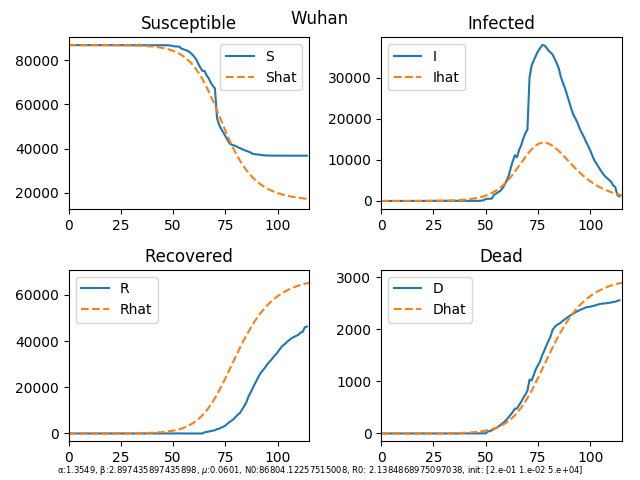
\includegraphics[width=\linewidth]{wuhan3.png}
  \caption{A boat.}
  \label{fig:boat1}
\end{figure}

Figure \ref{fig:boat1} shows a boat.


%\begin{figure}[h!]
%  \centering
%  \begin{subfigure}[b]{0.4\linewidth}
%    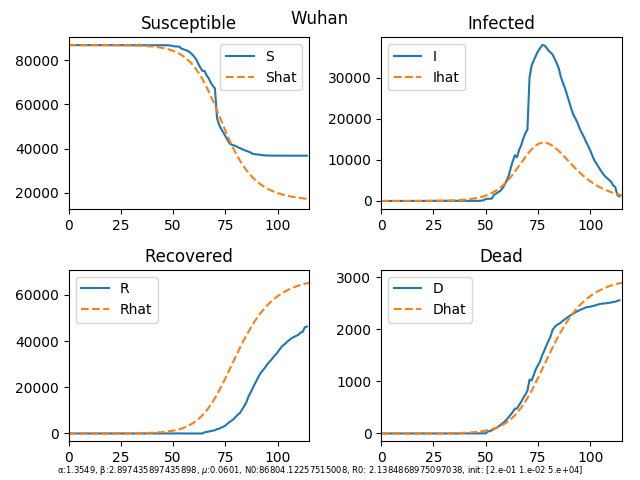
\includegraphics[width=\linewidth]{wuhan3.png}
%    \caption{Coffee.}
%  \end{subfigure}
%  \begin{subfigure}[b]{0.4\linewidth}
%   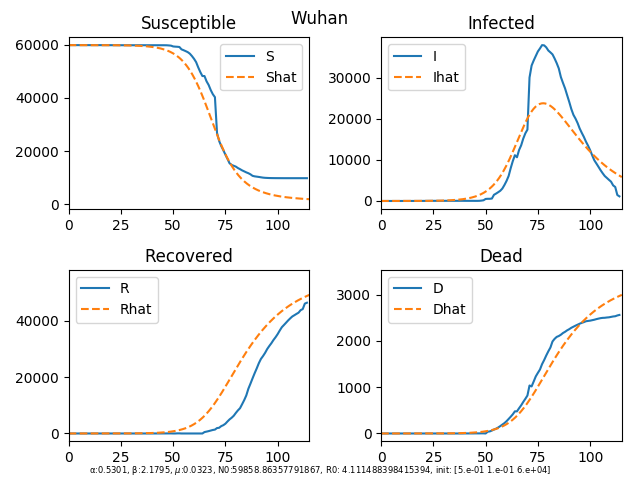
\includegraphics[width=\linewidth]{wuhan5.png}
%    \caption{More coffee.}
%  \end{subfigure}
%  \caption{The same cup of coffee. Two times.}
%  \label{fig:coffee}
%\end{figure}

\end{frame}

%%%%%%%%%%%%%%%%%%%%%%%%%%%%%%%%%%%%%%%%



\section{Data}

\begin{frame}{Main Data}
\textbf{Students}: 
\begin{itemize} 
	\item Data contains 152,350 students from 239 countries. 

\end{itemize}
\bigskip
\textbf{Schools}: 
\begin{itemize} 
	\item 1,739 institutions including 160 in Canada

\end{itemize}
\end{frame}




% All of the following is optional and typically not needed. 
\appendix
\section<presentation>*{\appendixname}
\subsection<presentation>*{References}

\begin{frame}
  \frametitle<presentation>{References}
    
  \begin{itemize}
  %\begin{thebibliography}{10}
    
  %\beamertemplatebookbibitems
  % Start with overview books.

  \item
    S. D.~Williamson.
    \newblock {\em Macroeconomics. Fifth Canadian edition. }.
    \newblock Don Mills, Ontario: Pearson Canada Inc
 \end{itemize}
    
  %\end{thebibliography}
\end{frame}

\end{document}

